\documentclass{article}
\usepackage{geometry}
\usepackage{hyperref}
\hypersetup{
    colorlinks=true,
    linkcolor=blue,
    citecolor=blue,
    }
\usepackage{amsmath}
\usepackage{amssymb}
\usepackage{algorithm}
\usepackage[noEnd=false]{algpseudocodex}
\usepackage{graphicx}
\graphicspath{ {./images/} }

\newtheorem{definition}{Definition}

\title{INF8750: BlindSort}
\author{Félix Larose-Gervais}

\pagestyle{headings}

\begin{document}
\maketitle
\newpage
\tableofcontents

\newpage

\section{Introduction}

\subsection{Motivation}

Currently, when a client needs some computation from a server, cryptography is often used to protect the client's data in transit. There will first be an asymmetric key exchange that will allow the client and server to agree on a key for symmetric encryption for the rest of the communication. This model protects the confidentiality of the user's data against an eavesdropper, however, the server decrypts and learn the user's data.

\begin{figure}[h]
    \centering
    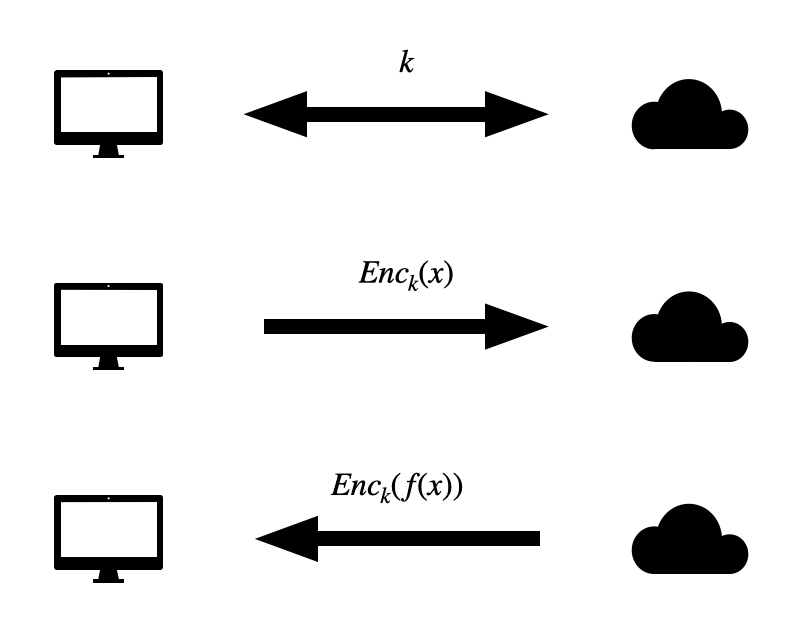
\includegraphics[scale=0.3]{dh}
    \caption{Key exchange followed by symmetric encryption}
\end{figure}

To enhance the user's privacy, we can use Fully Homomorphic Encryption (FHE). It allows computation to be made on ciphertexts without neeeding to decrypt them. This in turn enables building privacy preserving services that can act on their client's data without needing to see it in clear.

\begin{figure}[h]
    \centering
    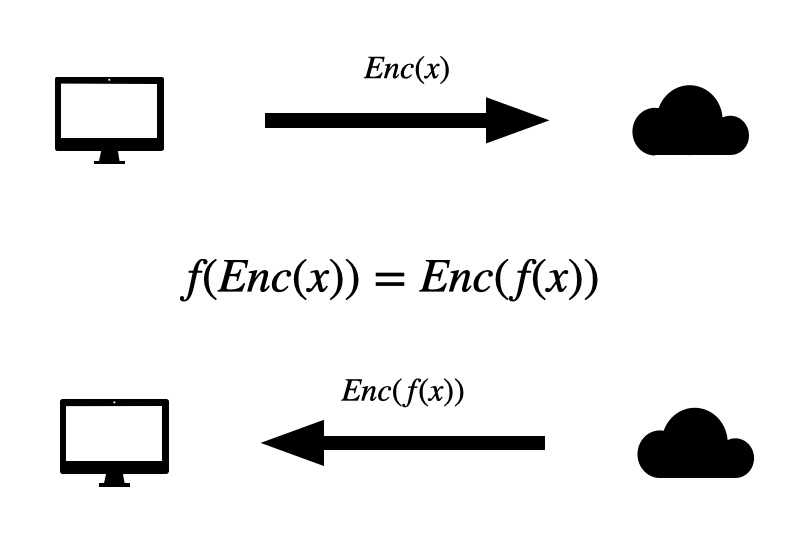
\includegraphics[scale=0.35]{fhe}
    \caption{Homomorphic encryption (The server doesn't learn the user's data)}
\end{figure}

Even though FHE has evolved a lot since its inception, its rather low performance is still hindering adoption. The goal of this project is to investigate performance of a modern FHE framework by implementing some sorting algorithms and comparing them with each other and the state of the art.

The first two algorithms are variants of the Direct Sort, first proposed by~\cite{lauter_depth_2015}. One using the Blind Matrix Access and Blind Permutation offered by RevoLUT~\cite{RevoLUT}, the other being a simple port of Direct Sort to TFHE-rs~\cite{TFHE-rs}. We also present a new algorithm based on two passes of Blind Permutation that speeds up the process significantly for certain types of arrays.

\newpage

\subsection{Homomorphic encryption}

Shortly after publishing the RSA cryptosystem~\cite{rivest_method_1978}, its authors noticed the scheme was in fact partially homomorphic~\cite{Rivest1978}. Then they asked whether a fully homomorphic encryption scheme was possible.

\begin{definition}
    A mapping $\varphi : \mathbb{G} \to \mathbb{H}$ is called an \textbf{homomorphism} if $\forall x, y \in \mathbb{G}$ we have:
    \[ \varphi(xy) = \varphi(x)\varphi(y)\]
\end{definition}

For example, $\varphi_q : \mathbb{Z} \to \mathbb{Z}_q$, $x \mapsto x \mod q$ is an homomorphism because it respects addition.

\begin{definition}
    An encryption scheme does \textbf{homomorphic encryption} if its encryption procedure is an homomorphism (modulo decryption).
\end{definition}

For example, an homomorphic encryption scheme $\Pi = (Gen, Enc, Dec)$ will satisfy:
\begin{align*}
    Enc(x + y) \equiv_{Dec} Enc(x) \oplus Enc(y)
\end{align*}

With respect to a $+$ a plaintext operation and its corresponding ciphertext operation $\oplus$.

\begin{definition}
    An encryption scheme is said to be \textbf{partially homomorphic} if it only allows certain computation on its ciphertexts without having to decrypt them.
\end{definition}

For example, the encryption scheme $RSA = (Gen, Enc, Dec)$ is partially homomorphic, because multiplications can be computed on ciphertexts.
\begin{align*}
    RSA = \begin{cases}
        Gen(1^n) &:= (N, e, d) \gets GenRSA \\
        Enc(m) &:= m^e \mod N \\
        Dec(c) &:= c^d \mod N
    \end{cases}
\end{align*}

Where $GenRSA$ computes $N = pq$ the product of two random primes and $e, d$ inverses in $\mathbb{Z}^{\times}_{\varphi(N)}$.

Given $m_1, m_2 \in \mathbb{Z}_N$, such that $c_1 = Enc(m_1)$ and $c_2 = Enc(m_2)$, we can verify:
\begin{align*}
    Enc(m_1m_2) 
        &\equiv {(m_1m_2)}^e \pmod N \\
        &\equiv m_1^e m_2^e \pmod N \\
        &\equiv Enc(m_1)Enc(m_2)
\end{align*}

We can see that decryption of the multiplication of ciphertexts yields the same result as multiplicating the corresponding plaintexts. Other cryptosystems have been shown to be partially homomorphic, notably~\cite{elgamal1985public},~\cite{benaloh1994dense} and~\cite{paillier1999}.

\begin{definition}
    An encryption scheme is said to be \textbf{fully homomorphic} if it allows any computation on its ciphertexts without having to decrypt them.
\end{definition}

The existence of a fully homomorphic encryption scheme was an open problem for 30 years. It was shown possible by~\cite{gentry_fully_2009}, who constructed the first fully homomorphic encryption scheme and presented a new idea, called bootstrapping, that allows to adapt some partially homomorphic schemes to make them fully homomorphic.

After his work, many fully homomorphic encryption schemes were proposed. In particular, TFHE~\cite{chillotti_tfhe_2020}, implemented in the TFHE-rs library, greatly improved performance over the initial construction.

\subsection{Fast Fully Homomorphic encryption over the Torus (TFHE)}

Fully Homomorphic Encryption over the Torus (TFHE)~\cite{chillotti_tfhe_2020} is a FHE scheme based on the Learning With Errors (LWE) problem. The security of the scheme is itself reduced to the difficulty of the Shortest Vector Problem (SVP) in lattices~\cite{regev_lattices_2009}.

For $p < q$ powers of two with $\Delta = q / p$, a message $m \in \mathbb{Z}_p$ can be encrypted into $(a, b) \in \mathbb{Z}_q^n \times \mathbb{Z}_q$
\begin{align*}
    LWE = \begin{cases}
        Gen(1^n) &:= s \overset{R}{\gets} {\{0, 1\}}^n \\
        Enc_s(m) &:= (a, \sum{a_i s_i} + \Delta m + e),\, a \overset{R}{\gets} \mathbb{Z}_q^n, e \overset{R}{\gets} \chi_\sigma \\
        Dec_s(a, b) &:= \lfloor b - \sum{a_i s_i} \rceil  / \Delta
    \end{cases}
\end{align*}

Where $a$ (the mask) is chosen uniformly at random and $e$ is sampled from a centered Gaussian distribution with standard deviation $\sigma$. We can verify this schema is additively homomorphic.
\begin{align*}
    Enc_s(m_1) + Enc_s(m_2) & = (a_1, a_1 \cdot s + \Delta m_1 + e_1) + (a_2, a_2 \cdot s + \Delta m_2 + e_2) \\
    &= (a_1 + a_2, (a_1 + a_2) \cdot s + \Delta (m_1 + m_2) + (e_1 + e_2)) \\
    &= Enc_s(m_1 + m_2)
\end{align*}

Similarly, we can encrypt arrays of fixed size $N$ (a power of 2) by encoding them as elements of $\mathcal{R}_q = \mathbb{Z}_q[X]/(X^N+1)$, that is the polynomials with integer coefficients (modulo $q$) of degree at most $N - 1$.
\begin{align*}
    RLWE = \begin{cases}
        Gen(1^n) &:= S \overset{R}{\gets} \mathcal{R}_2 \\
        Enc_s(M) &:= (A, AS + \Delta M + E),\, A \overset{R}{\gets} \mathcal{R}_q, E \overset{R}{\gets} \chi_\sigma \\
        Dec_s(A, B) &:= \lfloor B - AS \rceil / \Delta
    \end{cases}
\end{align*}

It's important to note that blind operations on the (R)-LWE ciphertexts accumulate noise. Therefore, after a certain amount of operations, that noise would overflow in the most significant bits that are reserved for the message, thus rendering the ciphertext un-decipherable. To solve this issue,~\cite{gentry_fully_2009} proposed the idea of bootstrapping; that is evaluating the decryption procedure homomorphically, given an encrypted key and doubly encrypted message. Repeating this procedure allows keeping the noise under a certain thresold.

\begin{figure}[h]
    \centering
    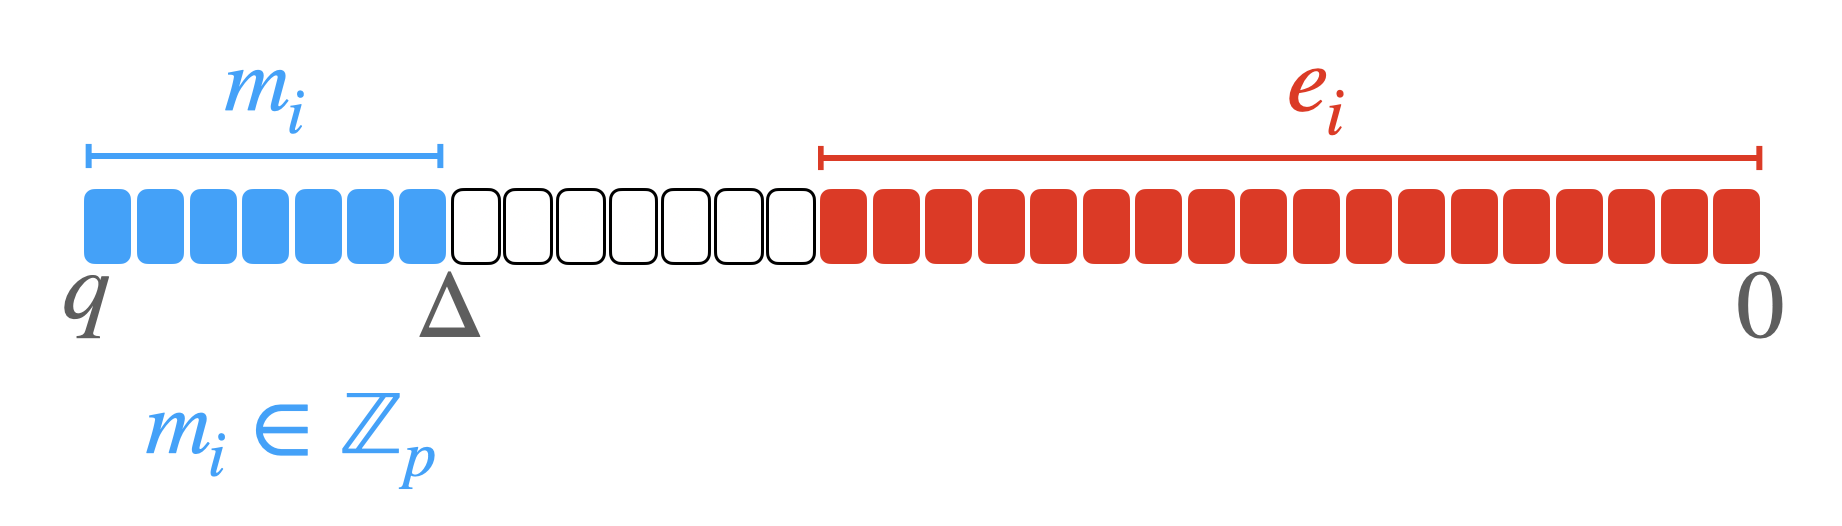
\includegraphics[scale=0.4]{lwe}
    \caption{Visual representation of a LWE ciphertext\cite{LWE}}
\end{figure}

\newpage

\subsection{RevoLUT}

The RevoLUT project, based on TFHE-rs, exposes a structure called a Look-Up Table (LUT). This structure is a fixed size array of ciphertexts, for which many new primitives where implemented such as blind permutation, blind array access and blind matrix access. These are all made possible thanks to TFHE's blind rotation, which is also at the core of their bootstrapping implementation.

\subsubsection*{Blind Rotation}

Blind Rotation is a primitive offered by TFHE-rs that allows to rotate a RLWE ciphertext by an encrypted integer amount. Given an encrypted polynomial $P = \sum{a_i X^i}$ and an encrypted integer $\alpha$, it computes $P X^{-\alpha}$. Due to the noise in $\alpha$ this operation is slightly inaccurate. To solve this, we introduce redundancy in the coefficients of the encrypted polynomials to accomodate for any noise.

\subsubsection*{Blind Array Access}

A Blind Array Access allows to access the encrypted coefficient of a LUT at an encrypted integer index $\alpha$. This is done by first performing a Blind Rotation of the LUT by $\alpha$, then a Sample Extraction (also provided by TFHE-rs) of the rotated LUT at index 0.

\subsubsection*{Blind Matrix Access}

A Blind Matrix Access allows to access the encrypted coefficient of an array of LUTs at an encrypted index $(\alpha, \beta)$. This is done by first performing a Blind Array Access into all the LUTs at index $\alpha$, packing the results into a new LUT and performing a Blind Array Access into this new LUT at index $\beta$.

\subsubsection*{Blind Permutation}

A Blind Permutation of a given LUT $T$ by an array of integer indices $\sigma$ is performed by obtaining the $n$ coefficients $T_i$ through Sample Extraction, and constructing $n$ LUTs starting with $T_i$, each rotating them blindly by the corresponding $\sigma_i$ and then summing the results into the output LUT.\@

\begin{figure}[h]
    \centering
    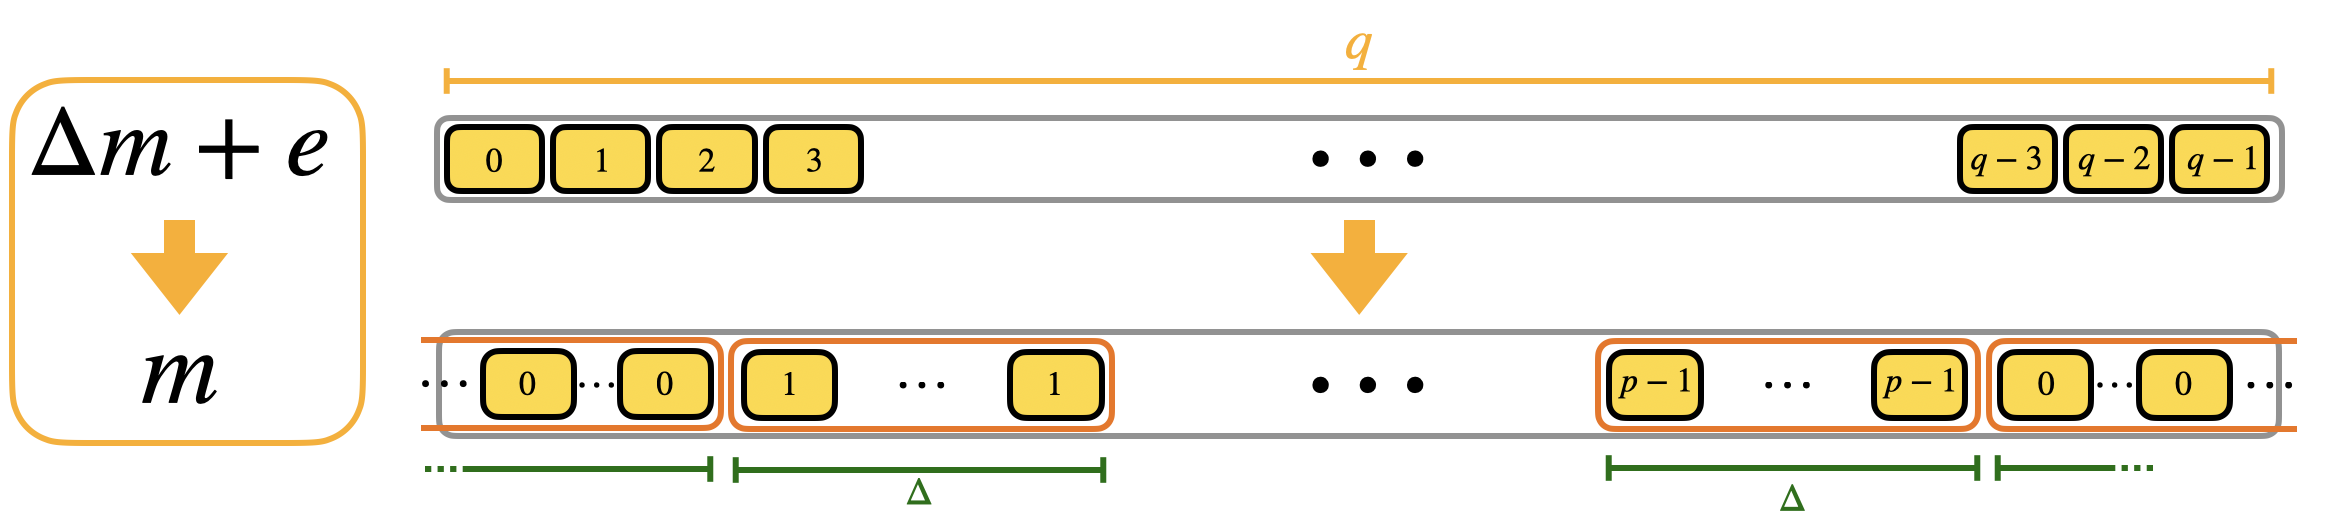
\includegraphics[scale=0.35]{lut}
    \caption{Visual representation of a LUT\cite{LUT}}
\end{figure}

\newpage

\section{Simple Sort}

\subsection{Main algorithm}

This first algorithm is the simplest, it is a variation of insertion sort documented in~\cite{fung2021simplest}. Its purpose is to serve as a baseline to compare to.

\begin{algorithm}
    \caption{Simple Sort}
    \begin{algorithmic}
        \Function{BlindSort}{T:\@ [FheUint]}
            \For{$i = 0$ to $n$}
                \For{$j = 0$ to $i$}
                    \State{$min = BlindMin(T_i, T_j)$}
                    \State{$max = BlindMax(T_i, T_j)$}
                    \State{$T_j \gets min$}
                    \State{$T_i \gets max$}
                \EndFor{}
            \EndFor{}
        \EndFunction{}
    \end{algorithmic}
\end{algorithm}

\subsection*{Notes}

It is interesting to see how easily certain algorithms can be ported to FHE. In this one, the indices being accessed in the array do not depend on the result of blind comparisons so implementation is pretty straightforward. 

It would have been desirable to also port an efficient algorithm to FHE for comparison purpose, but it is not as obvious how partition based algorithms like quicksort and mergesort would transfert. That is due to array accesses at indices depending on the result of blind comparisons.

\subsection{Implementation}

This algorithm was implemented using TFHE-rs, that already provides $BlindMin$ and $BlindMax$.

\subsection*{Analysis}

The procedure runs in $O(n^2)$ steps, each costing 2 blind operations. This makes the algorithm seem really inefficient. Despite this, it requires fewer blind operations than other more complicated algorithms presented after and therefore performs surprisingly well.

\newpage

\section{Direct Sort}

\subsection{Main algorithm}

The following is an adaptation of the direct sort proposed by~\cite{lauter_depth_2015}. The main idea of the algorithm is to construct a permutation from blind comparisons between pairs of elements of the given array, then apply it blindly.

\begin{algorithm}
    \caption{Direct Sort}
    \begin{algorithmic}
        \Function{BlindSort}{T:\@ [LWE]}
            \State{$\sigma \gets [0, \dots, 0]$}
            \For{$i = 0$ to $n$}
                \For{$j = 0$ to $i$}
                    \State{$b \gets BlindLt(T_i, T_j)$}
                    \State{$\sigma_i \gets \sigma_i + b$}
                    \State{$\sigma_j \gets \sigma_j + 1 - b$}
                \EndFor{}
            \EndFor{}

            \Return{$BlindPermutation(T, \sigma)$}
        \EndFunction{}
    \end{algorithmic}
\end{algorithm}

In the first step, we conceptually construct a comparison matrix $C = (C_{i, j})$ such that:
\begin{align*}
    C_{i, j} = \begin{cases}
        BlindLt(T_i, T_j) & \text{ if } i < j \\
        1 - C_{j, i} & \text{ otherwise }
    \end{cases}
\end{align*}

For example, given the LUT $T = [2, 1, 3, 2]$, we have:
\begin{align*}
    C &= \begin{pmatrix}
        0 & 1 & 0 & 0 \\
        0 & 0 & 0 & 0 \\
        1 & 1 & 0 & 1 \\
        1 & 1 & 0 & 0
    \end{pmatrix}
\end{align*}

We can view $\sigma = (1, 0, 3, 2)$ as the sums of the rows of the comparison matrix $C$.

Then, when applied to $T$ we get the sorted result $\sigma(T) = [1, 2, 2, 3]$.

\subsection*{Notes}

It is important to note that the blind comparison only happens for $i < j$. This was originally a performance concern due to the slowness of $BlindLt$ in RevoLUT (making only $\frac{n^2-n}{2}$ calls instead of $n$), but it ended up being important for correctness in arrays containing duplicates.

If $C$ was defined as $(C_{i, j})$ such that $C_{i, j} = BlindLt(T_i, T_j)$, we'd have:
\begin{align*}
    C &= \begin{pmatrix}
        0 & 1 & 0 & 0 \\
        0 & 0 & 0 & 0 \\
        1 & 1 & 0 & 1 \\
        0 & 1 & 0 & 0
    \end{pmatrix}
\end{align*}

Which would yield $\sigma = (1, 0, 3, 1)$ and would result in incorrect sorting.

\newpage

\subsection{Implementations}

\subsubsection*{RevoLUT}

$BlindLt(x, y)$ is defined as a $BlindMatrixAccess(L, x, y)$ with $L = {(i < j)}_{0 \leq i, j< n}$:
\begin{align*}
    L = \begin{pmatrix}
        0 & 0 & 0 & 0 \\
        1 & 0 & 0 & 0 \\
        1 & 1 & 0 & 0 \\
        1 & 1 & 1 & 0
    \end{pmatrix}
\end{align*}

The matrix $L$ is trivially encrypted; that is it's encrypted like with the LWE encryption procedure described earlier, except the mask $a$ is only zeroes instead of being sampled from a uniform distribution. This trivial encryption offers no security as it doesn't hide the message at all, but it allows running blind operations on it, and the result of those are properly confidential.

As for BlindPermutation, it is already implemented in RevoLUT.\@

\subsubsection*{TFHE-rs}

This second implementation works very similarly to the first one, except that $BlintLt$ is already provided by TFHE-rs, but not $BlindPermutation$. It can be implemented like~\cite{lauter_depth_2015} in the following way:

\begin{algorithm}
    \caption{Blind Permutation in TFHE-rs}\label{BlindPermutation}
    \begin{algorithmic}
        \Function{BlindPermutation}{T:\@ [TfheUint], $\sigma$: [TfheUint]}
            \State{$R \gets [0, \dots, 0]$}
            \For{$i = 0$ to $n$}
                \For{$j = 0$ to $n$}
                    \State{$R_i \gets R_i + BlindEq(\sigma_j, i) \times T_j$}
                \EndFor{}
            \EndFor{}

            \Return{R}
        \EndFunction{}
    \end{algorithmic}
\end{algorithm}

$BlindEq$ is provided by TFHE-rs.

\subsubsection*{Analysis}

The main differences between the two implementations are in the algorithmic complexities of $BlindLt$ and $BlindPermutation$.

For RevoLUT, $BlindLt \in O(n^2)$ because $BlindMatrixAccess$ requires $n + 1$ blind rotations, each of which are linear in $n$. $BlindPermutation \in O(n^2)$ because it requires $n$ blind rotations. This totals to $O(n^4)$.

However, in the second implementation, because the blind comparisons are implemented as bivariate functions over radix integers, they are essentially logarithmic in $n$. Thus, we have $BlindLt \in O(\log(n))$ and $BlindPermutation \in O(n^2 \log(n))$. That makes the whole procedure run in time $O(n^2\log(n))$.

\newpage

\section{Double Blind Permutation}

\subsection{Main algorithm}

The idea of this third algorithm is to interpret the given array as a permutation, apply it to itself to get a partially ordered sparse array. Then fix it by percolating null values to the end.

\begin{algorithm}
    \caption{Permutation Sort}
    \begin{algorithmic}
        \Function{BlindSort}{T:\@ [LWE]}
            \State{$R \gets BlindPermutation(T, T)$}
            \State{$\sigma \gets [0, \dots, 0]$}
            \State{$z \gets 0$}
            \For{$i = 0$ to $n$}
                \State{$z \gets z + BlindEq(R_i, 0)$}
                \State{$\sigma_i \gets R_i - z$}
            \EndFor{}

            \Return{$BlindPermutation(R, \sigma)$}
        \EndFunction{}
    \end{algorithmic}
\end{algorithm}

For example, given an array \[T = [5, 2, 7, 3, 0, 0, 0, 0]\]

We can construct \[\sigma_1 = (5, 2, 7, 3, 0, 0, 0, 0)\]

And apply it to itself to get \[R = \sigma_1(T) = [0, 0, 2, 3, 0, 5, 0, 7]\]

Then we conceptually construct $Z$ such that $Z_i$ counts zeroes in $R$ up to (and including) $i$ \[ Z = [1, 2, 2, 2, 3, 3, 4, 4] \]

We compute $\sigma_2 = R - Z \mod n$ \[ \sigma_2 = (7, 6, 0, 1, 5, 2, 4, 3) \]

And then finally we return $BlindPermutation(R, \sigma_2)$ \[ \sigma_2(R) = [2, 3, 5, 7, 0, 0, 0, 0]\]

\subsection*{Notes}

There are a few limitations to this approach. First, it doesn't work on duplicate entries in its current form (the first permutation will lose information). Secondly, it doesn't consider $0$ as a value provided by the user.

\newpage

\subsection{Implementations}

\subsubsection*{RevoLUT}

$BlindPermutation$ is already implemented in RevoLUT.\@ And $BlindEq(R_i, 0)$ can be expressed as $BlindArrayAccess(L, R_i)$ for the trivially encrypted $L = [1, 0, \dots, 0]$.

\subsubsection*{TFHE-rs}

$BlindPermutation$ as defined earlier in Algorithm~\ref{BlindPermutation} can be re-used here, and $BlindEq$ is already provided by TFHE-rs. That makes this implementation fairly straightforward.

\subsubsection*{Analysis}

For the first implementation, recall that $BlindPermutation \in O(n^2)$ in RevoLUT, and the $n$ passes of the linear $BlindEq$ add up to a total of $O(n^2)$.

As for the second, the middle loop clocks in at a faster $O(n\log(n))$ thanks to TFHE-rs' fast bivariate functions, but the whole time is dominated by the 2 slower blind permutation that are running in $O(n^2\log(n))$.

\begin{figure}[h]
    \centering
    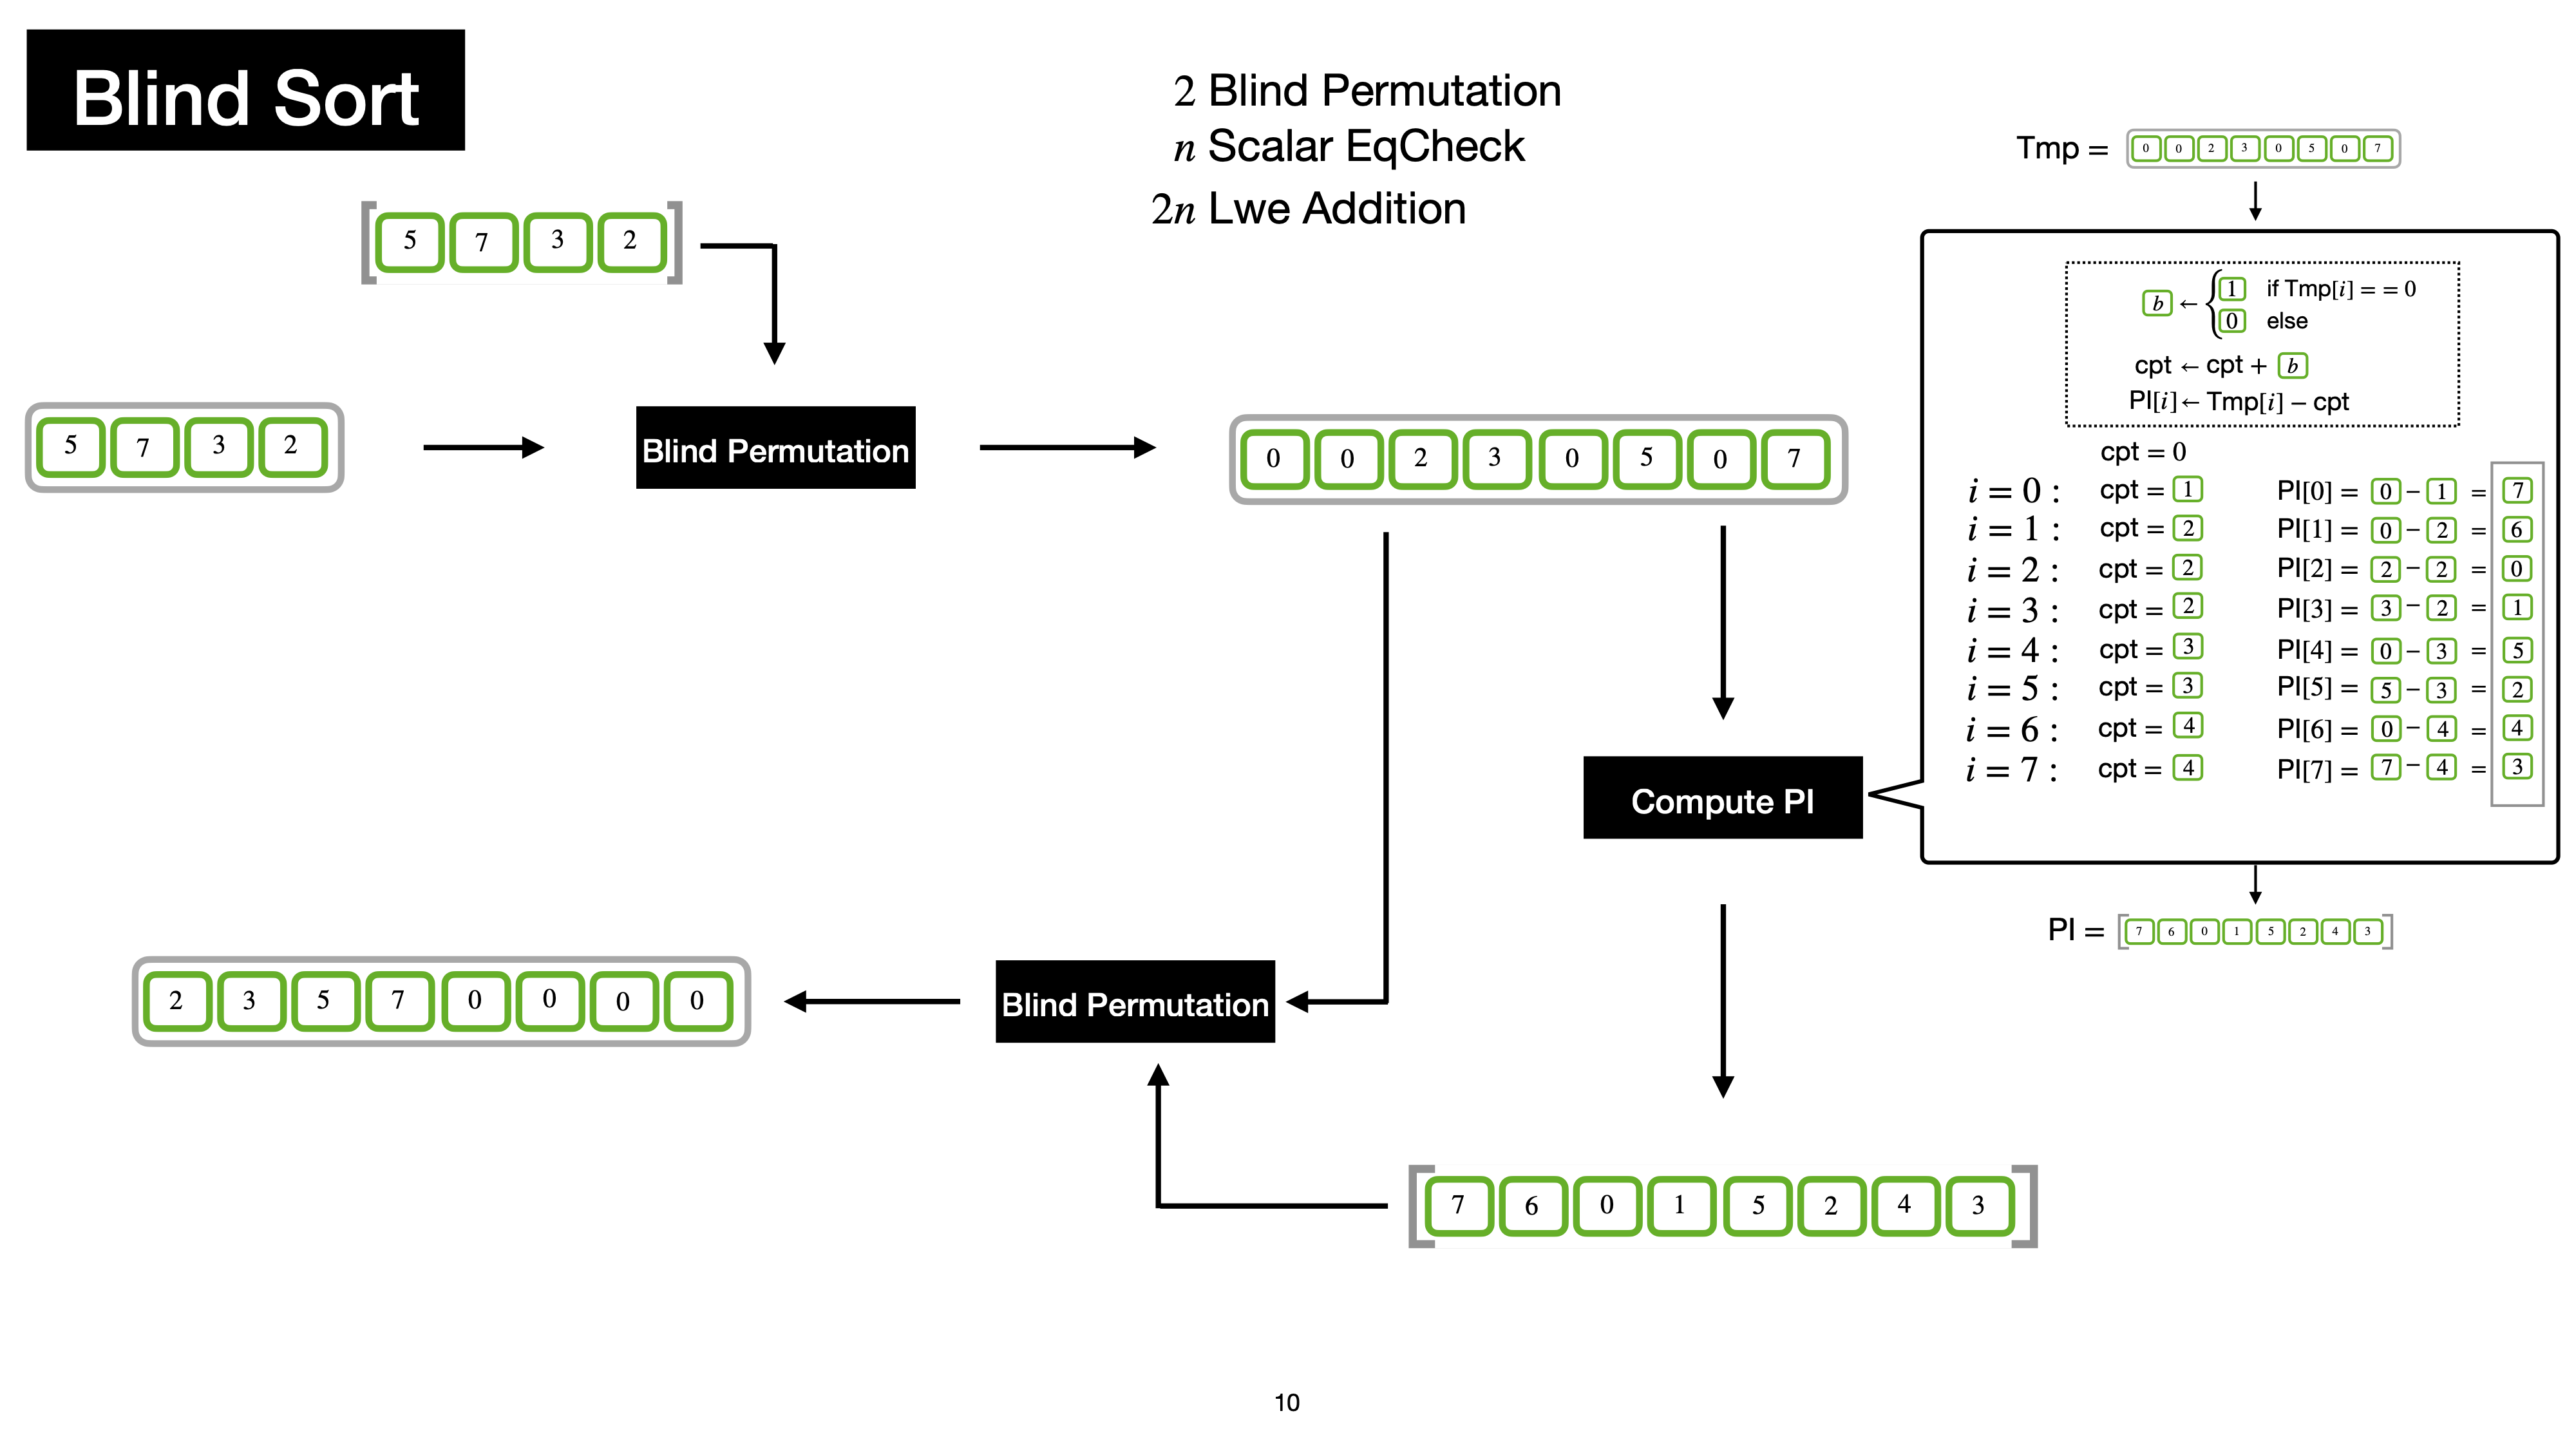
\includegraphics[scale=0.1]{2bp}
    \caption{Illustration of the Double Blind Permutation sorting algorithm}
\end{figure}

\newpage

\section{Results}

\subsection{Methodology}

To compare the performance of the different sorting algorithms implemented, we used the statistics-driven micro-benchmarking framework Criterion. Multiple runs of randomly generated encrypted arrays of various sizes where sorted with all implementations.

Also, the Blind Permutation of RevoLUT is compared to the naive one we implemented in TFHE-rs to gain insights on the performance characteristics of the two sorting algorithms.

\subsection{Benchmarks}

The first two figures are extracted from the cited papers, other numbers where obtained by running the experiment code available on github.com at filedesless/blindsort and sofianeazogagh/revoLUT.\@ The experiments were ran on a 13-inch macbook pro m1 2020.

\begin{center}
    \begin{tabular}{|l||c|c|c|c|}
        \hline
        & \multicolumn{4}{|c|}{Array Size} \\
        \hline
        & 4 & 8 & 16 & 32 \\
        \hline
        Direct Sort (\cite{lauter_depth_2015}) & 500ms & 5s & 50s & 7m \\
        Direct Sort (\cite{iliashenko_faster_2021}) & 80ms & 700ms & 6s & 50s\\
        \hline
        Direct Sort (RevoLUT) & 2s & 20s & 2m & -\\
        Direct Sort (TFHE-rs) & 2s & 10s & 40s & 2m\\
        \hline
        Naive Blind Permutation (TFHE-rs) & 1s & 4s & 16s & 1m\\
        RevoLUT Blind Permutation (RevoLUT) & 400ms & 800ms & 3.6s & 10s\\
        \hline
        Double Blind Permutation (THFE-rs) & 3s & 9s & 33s & 2m\\
        Double Blind Permutation (RevoLUT) & 1s & 2s & 5s & 21s\\
        \hline
        Simple Sort (TFHE-rs) & 1s & 5s & 23s & 104s \\
        \hline
    \end{tabular}
\end{center}

\subsection{Remarks}

First we can observe that even though Blind Permutation is faster within RevoLUT than TFHE-rs, this isn't enough to overcome the slowness of the Blind Matrix Access used in the Blind Comparison. However, it makes a great difference for the second algorithm where we get very interesting figures.

The Double Blind Permutation shows promising results, being much faster than the state of the art. However, there is still some outstanding issues that need to be resolved and the numbers from the papers should be reproduced on the same hardware to obtain a more fair comparison.

Finally, the most surprising result was the relative performance of Simple Sort. This is probably due to the fewer blind operations being performed in total.

\newpage

\section{Conclusion}

In conclusion, the results show that the fastest proposed algorithm is the Double Blind Permutation, implemented with RevoLUT's fast Blind Permutation.

\subsection{Caveats}

However, the algorithm is limited to sorting distinct non null values. We have some ideas to extend it, but at an unclear performance cost. In order to support duplicates, we would have to somehow count them and adjust the permutations accordingly.

It would also be nice to run the state of the art benchmarks on the same hardware as our proposed solution. Currently, timing numbers are being compared from different sources which is fairly inaccurate.

\subsection{Future work}

Other research avenues include investigating the feasability of porting partition based sorting scheme like quicksort or mergesort to FHE.\@ The indices being accessed in the encrypted array depending on the result of blind operations make this non-obvious, but there might be a way to use Blind Rotations to achieve the same effect at a reasonable performance cost.

Another interesting option is to consider non comparison based sorting algorithms like counting sort. The fixed size nature of RevoLUT seem to make it a good candidate for algorithms whose complexity depends on the size of the structure and the size of the stored elements.

\bibliography{refs}
\bibliographystyle{apalike-uqam}

\end{document}